% !TeX root = ../main.tex

\chapter{石墨烯的超导特性(魔角二层、魔角三层、菱面体三层石墨烯)及其潜在应用}

BCS理论是经典的、传统的超导理论,使用弱电子-声子相互作用(weak electron–phonon interactions)模型,能解释很多固体的低温(液氦)超导;但随着越来越多的超导体被发现,人们发现BCS理论并不能解释所有超导体;这类不能被解释的超导体称作非常规超导体(unconventional superconductor)。近些年,石墨烯在科研中是一种很重要的二维非常规超导体。

\section{超导的相关概念}

最早发现的超导体是铜氧超导体,由它开始,人类揭开了常规超导体的面纱。伴随着研究的深入,这种突破了常规理论的导电现象逐渐有了一套相对成熟的理论解释——BCS理论。

BCS理论以近自由电子模型为基础,提出者是巴丁(J.Bardeen)、库珀(L.V.Cooper)、施里弗(J.R.Schrieffer)。理论认为,金属中自旋和动量相反的电子可以配对形成库珀对(Cooper pair)(也称库珀电子对,美国物理学家 Leon Cooper于1956年首次提出),库珀对在晶格当中可以无损耗的运动,形成超导电流。对于库珀对产生的原因,BCS理论做出了如下解释:电子在晶格中移动时会吸引邻近格点上的正电荷,导致格点的局部畸变,形成一个局域的高正电荷区。这个局域的高正电荷区会吸引自旋相反的电子,和原来的电子以一定的结合能相结合配对(称作以弱耦合形式形成)。在很低的温度下,这个结合能可能高于晶格原子振动的能量,这样,电子对将不会和晶格发生能量交换,没有电阻,没有能量损失,形成超导电流。

科学家使物质实现超导性主要通过降低温度和施加电场。由于库珀电子对作用很弱,热能很容易打破库珀电子对的相互作用,因此需要降低温度;而施加电场会改变能带结构,使得大量具有不同动量值的电子可以填充狭窄的能级范围,加强了电子对中电子之间的相互作用。也正是由于这样的原因,常规超导体很难实现常温超导。

此外,关于BCS理论中的库珀对(称作自选单线态库珀对,即自旋相反),还有这样一种效应会打破它们的相互作用:塞曼效应(Zeeman effect)。它使得在称为泡利极限(Pauli limit)的磁感应强度之上时,自旋指向同一方向;随着自旋改变,自旋单线态库珀对被打破,超导性消失。

\section{石墨烯超导性质}

\subsection{魔角扭曲双层石墨烯}

扭曲双层石墨烯(twisted bilayer graphene),是将两片堆叠的石墨烯片扭转一小角度形成的。扭转“魔角“时费米速度降为0(能带结构零费米能),(理论上)预测的第一个魔角为1.1°,这样的扭转双层石墨烯亦即魔角扭曲双层石墨烯(magic-angle twisted bilayer graphene,亦即MATBG)。魔角石墨烯半填充时呈绝缘状态,静电掺杂使之远离绝缘状态后,它呈零电阻;临界温度可达1.7K。

\begin{figure}
    \centering
    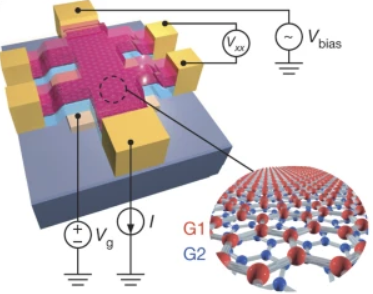
\includegraphics[scale=0.7]{img/魔角双层.png}
    \caption{典型双层双分子墨烯(TBG)器件和四探针(V)的示意图}
\end{figure}

MATBG的性质与表征:

\begin{itemize}
    \item 扭曲双层石墨烯的温度 - 载流子密度相图与铜氧超导体的温度 - 载流子密度相图相似,并包括对应于超导性的圆顶形区域
    \item 材料纵向电阻中的量子振荡表明在相关绝缘态附近存在小费米表面,类似于低掺杂铜氧超导体
\end{itemize}

\smallskip

MATBG意义:

\begin{itemize}
    \item 库珀对中电子间作用力最强的超导体
    \item 第一个精确可控、纯碳基2D超导体
    \item 可以再现地测量鲁棒超导性(一种稳定的超导性)的石墨烯材料
    \item 唯一一个超导在虽低温、但载流子浓度低的条件下实现,这个性质暗示着投入实际应用有很大前景
    \item 它承载了丰富多样的相关量子相,是研究强关联现象、高临界温度超导体和量子自旋液体的理想材料
\end{itemize}

\begin{figure}
    \centering
    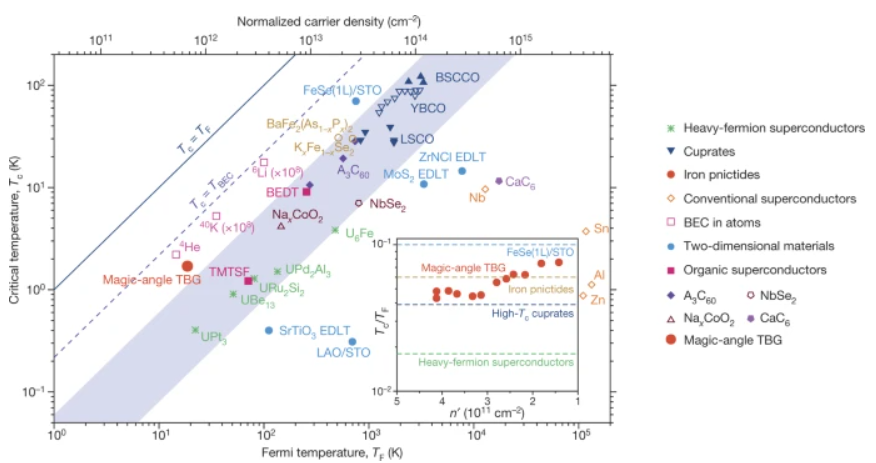
\includegraphics[scale=0.5]{img/载流子密度.png}
    \caption{各种不同超导体$T_c/T_F$图}
\end{figure}

\section{魔角扭曲三层石墨烯}

将三片堆叠的石墨烯片对称地扭转一小角度(如下图),就形成扭曲三层石墨烯;同样地,扭转“魔角“(如1.6°)时费米速度降为0,此时的扭曲三层石墨烯称作魔角扭曲三层石墨烯(magic-angle twisted trilayer graphene,亦即MATTG)。MATTG在1K以下被发现为moiré超导体,其电子结构和超导性能比魔角扭曲双层石墨烯具有更好的可调控性。

\begin{figure}
    \centering
    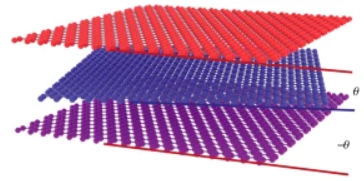
\includegraphics[scale=0.8]{img/魔角扭曲三层石墨烯.png}
    \caption{MATTG结构}
\end{figure}

MATTG的性质、表征与相关讨论:

\begin{itemize}
    \item 临界磁感应强度(随磁场增强,超导性消失的磁感应强度)高达10T,对传统自旋单线态超导体的泡利极限有很大出入(2-3个数量级),这些性质与传统的自旋单线态超导体迥然不同,推测MATTG中的库珀对为自旋三线态(即自旋相同,与BCS理论矛盾)电子对;(注:这一点需要通过进一步实验数据来验证)

          \begin{figure}
              \centering
              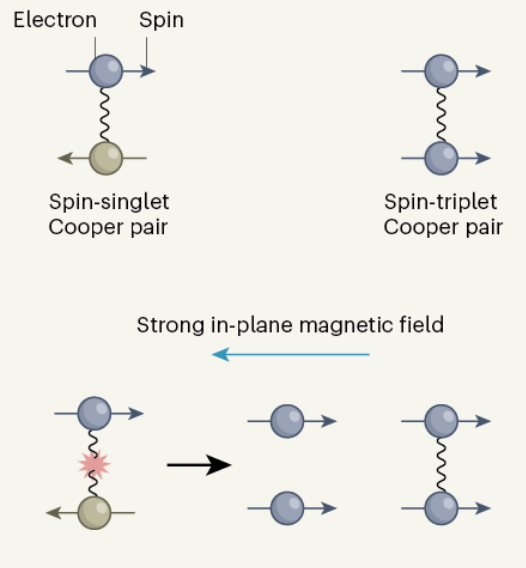
\includegraphics[scale=0.6]{img/自旋.png}
              \caption{MATTG库珀对的自旋状态}
          \end{figure}

    \item 在强磁场下、较窄的载流子密度和位移场范围内,随着磁场增大,观察到超导性的消失后又重现了(称为第二超导相),这和以前发现的碲化铀性质相近,表明魔角扭曲三层石墨烯中的超导性很可能是由导致非自旋单线库珀对的机制驱动的,并且外部磁场可以引起具有潜在不同顺序参数的相之间的跃迁
    \item 零磁场电阻率测量表明,超导的存在与每个moiré晶胞的两个载流子产生的破碎对称相密切相关,超导相在部分围绕破碎对称相的范霍夫奇点(Van Hove singularitie)处被抑制和限制,这很难用持弱耦合作用观点的BCS理论来解释
    \item MATTG系统广泛的原位可调性使之能够达到超强耦合状态,其特征是金茨堡-朗道相干长度(Ginzburg–Landau coherence length)达到平均粒子间距离,并且具有非常大的$T_{BKT}/T_F$值,超过 0.1(其中$T_{BKT}$和$T_F$分别是Berezinskii-Kosterlitz-Thouless跃迁温度和费米温度)
\end{itemize}

\begin{figure}
    \centering
    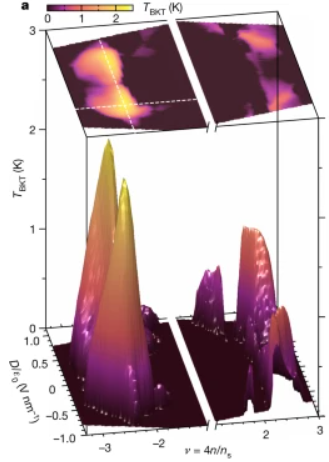
\includegraphics[scale=0.3]{img/三维图.png}
    \caption{图为MATTG的TBKT-D-ν三维图,其中D为电位移,$ν=4n/n_s$}
\end{figure}

意义:

\begin{itemize}
    \item 为可以通过实验操纵的非常规超导体铺平了道路
    \item 可以从弱耦合到强耦合范围内调控库珀电子对的作用
    \item 有可能彻底改变对强耦合超导的基本理解
    \item 证明了moiré超导性的丰富性
    \item 指导下一代奇异量子物质的设计\cite{RN49,RN50,RN51}
\end{itemize}

\section{菱面体三层石墨烯}

菱形三层石墨烯(rhombohedral trilayer graphene,简称RTG)是一种亚稳态的、自然界存在的碳的同素异形体(扭曲石墨烯需要人工合成),结构上比扭曲石墨烯稳定,在实验中无序性低于扭曲石墨烯。在亚开尔文温度(106mK),在电场下,菱面体三层石墨烯也实现了超导。超导性发生在两个不同的栅极调谐区域(SC1和SC2),并且净极限(clean limit)很深\footnote{净极限定义:平均自由程和超导相干长度(superconducting coherence length)之比}。

\begin{figure}
    \centering
    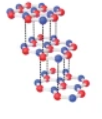
\includegraphics[scale=1.5]{img/3.png}
    \caption{RTG结构}
\end{figure}

菱面体三层石墨烯的性质、表征与相关讨论:

(1)电子行为研究

i.当添加额外的电子时,系统能量的变化,测量其电阻和电子可压缩性,可表现出多种电子基态:通常,可压缩性是正的,因为系统的能量随着每个电子的增加而增加;然而,当电场和电子密度改变时,他们检测到多个正可压缩性区域,这些区域由负可压缩性的边界隔开,这表明了不同电子基态之间的相变;

ii.进一步地,系统对面内和面外磁场的响应指出了这些相:电子具有固有的磁矩,分为自旋向上或向下(当电子不相互作用时,能量上的稳态具有相等的自旋向上和自旋向下的电子数目,导致净磁矩为0);同时,电子也可以通过其能带结构中的两个最小值来表征,称为它们的谷自由度(valley degree),取值K和K′;这四种状态——(up,K)、(up、K′)、(down、K)和(down,K′)——共同定义了电子的同位旋(isospin);

iii.在菱形三层石墨烯中,当载流子密度很高时,所有四种同位旋状态比例等表示,产生没有净磁矩的对称相;低载流子密度下则呈两个不同的铁磁性相,自旋和谷自由度都取了一个值,称作四分之一金属相(自旋、谷自由度组合采用四种可能性中的任意一种状态);在载流子密度适中时,出现半金属相:其中所有电子自旋都指向相同的方向,但谷自由度K和K′分布均匀;不同地,大多数传统铁磁体中也存在两种类型的自旋,但比例不同。(如下图)

\begin{figure}
    \centering
    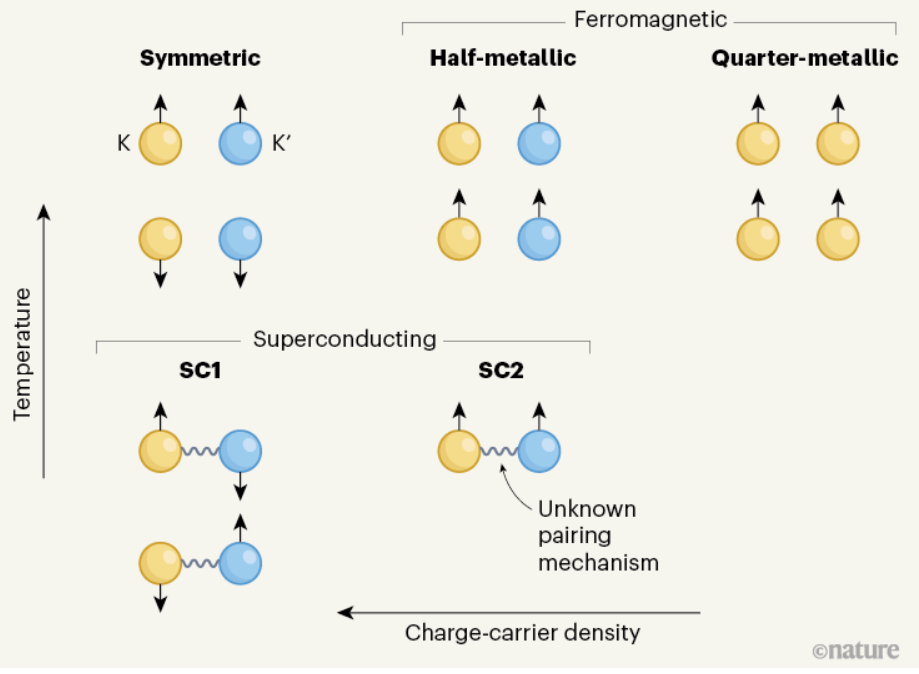
\includegraphics[scale=0.6]{img/4.png}
    \caption{库珀对电子同位旋示意图,黄表示K,蓝表示K’}
\end{figure}

iv.菱面体三层石墨烯与魔角扭曲三层石墨烯的电子可压缩性表征基本一致,唯一的差异在于扭曲引入的能带结构中的额外能量间隙;二者具有相似的铁磁性和超导性,这暗示着这两种性质背后的密切联系;

v.这些相的确定有待于进一步实验验证,例如:测量安德烈耶夫反射(Andreev reflection),这将证明即使在没有磁场的情况下,自旋在四分之一和半金属相中也是完全一致;

(2)通过量子振荡绘制法线态(normal state)费米表面图,该面表征了在费米能级下电子的动量,表明两个超导相都来自环形费米海(Fermi sea),并且在等旋对称断裂跃迁的近端,费米表面发生简并化,研究人员假设,有序状态的波动(如自旋)可能会由介导配对机制调节;

\begin{figure}
    \centering
    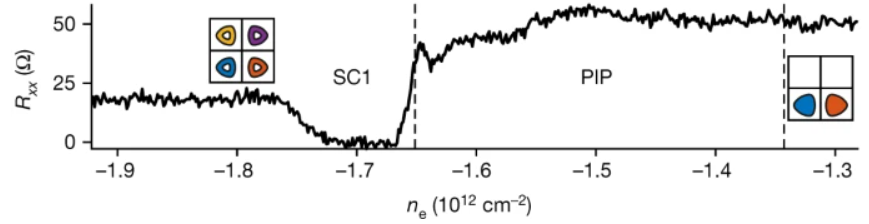
\includegraphics[scale=0.4]{img/5.png}
    \caption{费米表面图}
\end{figure}

(3)SC1在顺磁法态(paramagnetic normal state)出现,降低温度时对称相中变化得到,而SC2在自旋极化(spin-polarized)、非极化谷态(valley-unpolarized)中出现,降低温度时从半金属相变化得到。其中,SC1的泡利极限为300mT,符合传统的理论;但SC2为1T,至少常规超导体泡利极限一个数量级,与魔角三层石墨烯一样,表明此时库珀对可能是自旋三线态。

意义:

\begin{itemize}
    \item 为纯净且结构简单的二维金属(two-dimensional metal)中的超导性的观察提供了一个模型系统,可以测试不同的的超导理论模型,不会出现复杂的建模障碍
    \item 使基于相关电子现象和弹道电子传输的新型场效应控制电子设备成为可能
    \item 电子的相是电子的固有性质,RTG只是一个现实存在的理想的载体,在载体中电子的相很容易被表征出来\cite{RN53,RN54}
\end{itemize}

\section{石墨烯超导性研究的总体意义}

科学家们已经发展出了“转角电子学”这样一个领域,通过扭转两层石墨烯的角度,去寻找电子运动的普遍规律。这个研究实际上为材料学打开了新思路,那就是,材料学可以根据物质性质的底层逻辑进行预测和构建。

此外,其他很多凝聚态物理、自旋物理学的科学前沿理论也依赖于石墨烯超导的研究来验证或证伪,这项研究对前沿领域理论的发展和完善具有重要意义。

\section{石墨烯超导性的潜在应用}

\subsection{二维自旋三线态超导}

由前文所述,在MATTG和RTG中发现了二维自旋三线态超导现象(有待进一步确认)。而据预测,其中许多二维自旋三线态超导体会受到“马约拉纳零模式”(Majorana zero mode)的奇异零能量激发;一个成熟的例子是2D手性p-波超导体(chiral p-wave superconductor),该系统打破了时间反转对称性(如果时间方向相反,其物理性质会发生变化),并且当垂直于系统施加磁场时,预计马约拉纳零模式将存在于磁通量线程涡旋的中心。马约拉纳零模式是拓扑量子比特——拓扑量子计算的“容错”量子计算的构建模块——的潜在载体。如今,大多数已知的自旋三线态超导体是3D的,因此实验建立的2D自旋三线态超导体是非常需要的。然而,自旋三线态的发现并不一定意味着能实际应用于拓扑量子计算,需要进一步研究超导的拓扑性质,如,它是否能打破了时间反转对称性,涡旋中心中零能量状态的直接证据是否能寻找到(进而表明马约拉纳零模式的存在),等等。\cite{RN51}

\subsection{常温超导}

由前所述,常规超导在常温条件下必然失去超导性。因此,想要提高临界温度,必须从非常规超导出发。这也是超导应用研究的一大热门方向。

虽然石墨烯的几篇论文的温度都是在低温下的,离传统应用的方向较远;但一般常温超导体有莫特绝缘态\cite{RN54},魔角石墨烯也符合这一点(虽然有争议,有物理学家表示可以不用这个模型解释),且载流子浓度低,有极大可能可能发展成常温超导。

如果常温超导实现了,再在考虑消除超导体其他性质的影响后,如果材料成本合适,有望取代银和铜,作为导线,减少能量损耗。超导体的磁学性质使常温超导也有望应用于磁悬浮列车。
此外,超导体应用方向还有:超导发电机、超导电磁推进系统、聚能武器等,这些应用已有了一定发展,未必使用常温超导,但无疑常温超导更有利于减小这些应用的成本。

由铊-钡-钙-铜-氧超导薄膜(一种铜氧超导体)制成的装置,已应用于移动电话的发射塔,以增加容量,减少断线和外界干扰;而MATTG类似于铜氧超导体的性质,也同样能有望替代之。